\documentclass[12pt,aspectratio=169]{beamer}
\usetheme{metropolis}
\setbeamersize{text margin left=.5cm,text margin right=.5cm}
\usepackage[lf]{carlito}
\usepackage{tikz}
\usepackage{mathpazo}
\usepackage{xcolor,colortbl}
\usepackage{siunitx}
\usepackage{circuitikz}

\setlength{\parskip}{0pt}
\renewcommand{\baselinestretch}{1}

\sisetup{
  per-mode=symbol
}
\tikzset{>=latex}

\title{Topic 12: Capacitors}
\subtitle{Advanced Placement Physics 2}
\author[TML]{Dr.\ Timothy Leung}
\institute{Olympiads School}
\date{Last Updated: \today}

\newcommand{\pic}[2]{\includegraphics[width=#1\textwidth]{#2}}
\newcommand{\mb}[1]{\mathbf{#1}}
\newcommand{\eq}[2]{\vspace{#1}{\Large\begin{displaymath}#2\end{displaymath}}}


\begin{document}

\begin{frame}
  \maketitle
\end{frame}


\section{Capacitors}


\begin{frame}{Electric Field and Electric Potential Difference}
  \begin{center}
    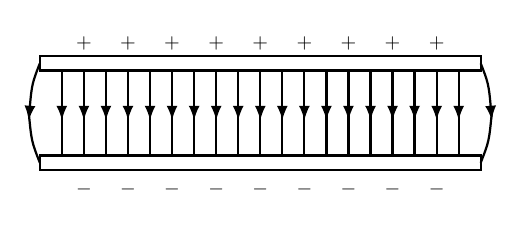
\begin{tikzpicture}[xscale=.7,yscale=.9]
      \draw[thick](0,0) rectangle (8,.2);
      \draw[thick](0,1.4) rectangle (8,1.6);
      \foreach\x in {.4,.8,1.2,...,7.6}{
        \draw[->,thick](\x,1.4)--(\x,.7);
        \draw[thick](\x,1.4)--(\x,.2);
      }
      \foreach\x in {.8,1.6,2.4,...,7.2}{
        \node at (\x,1.78) {\scriptsize $+$};
        \node at (\x,-.28) {\scriptsize $-$};
      }
      
      \draw[->,thick](0,1.5)..controls(-.15,1.2)..(-.2,.7);
      \draw[thick](-.2,.8)..controls(-.15,.4)..(0,.1);

      \draw[->,thick](8,1.5)..controls(8.15,1.2)..(8.2,.7);
      \draw[thick](8.2,.8)..controls(8.15,.4)..(8,.1);
    \end{tikzpicture}
  \end{center}
  \vspace{-.1in}Recall that the electric field between two (infinitely) large
  parallel plates is uniform, and the relationship between electric field and
  voltage is given by:

  \eq{-.2in}{
    \boxed{E=\frac Vd}
  }
  \begin{center}
    \begin{tabular}{l|c|c}
      \rowcolor{pink}
      \textbf{Quantity} & \textbf{Symbol} & \textbf{SI Unit} \\ \hline
      Electric field intensity & $E$ & \si{\newton\per\coulomb}\\
      Electric potential difference between plates & $V$ & \si{\volt} \\
      Distance between plates                      & $d$ & \si{\metre}
    \end{tabular}
  \end{center}
\end{frame}



\begin{frame}{Capacitors}
  \textbf{Capacitors} is a device that stores energy in an electric field. The
  simplest form of a capacitor is a set of closely spaced parallel plates:
  \begin{center}
    \pic{.5}{cap19}
  \end{center}
  When the plates are connected to a battery, the battery transfer charges to
  the plates until the voltage $V$ equals the battery terminals. After that,
  one plate has charge $+Q$; the other has $-Q$.
\end{frame}



\begin{frame}{Parallel-Plate Capacitors}
  As we have seen already, the (uniform) electric field between two parallel
  plates is proportional to the charge density $\sigma$, which is the charge
  $Q$ divided by the area of the plates $A$:

  \eq{-.2in}{
    E=\frac{\textcolor{red}{\sigma}}{\epsilon_0}=
    \frac{\textcolor{red}{Q}}{\textcolor{red}{A}\epsilon_0}
  }
  
  Substituting this into the relationship between the plate voltage $V$ and
  electric field, we find a relationship between the charges across the plates
  and the voltage:

  \eq{-.2in}{
    V=\textcolor{blue}{E}d=
    \frac{\textcolor{blue}{Q}d}{\textcolor{blue}{A\epsilon_0}}
    \quad\longrightarrow\quad
    \boxed{Q=\left[\frac{A\epsilon_0}{d}\right]V}
  }
\end{frame}



\begin{frame}{Parallel-Plate Capacitors}
  Since area $A$, distance of separation $d$ and the vacuum permittivity
  $\epsilon_0$ are all constants, the relationship between charge $Q$ and
  voltage $V$ is \emph{linear}. And the constant is called the
  \textbf{capacitance} $C$, defined as:

  \eq{-.15in}{
    \boxed{C=\frac{Q}{V}}
  }

  For parallel plates:

  \eq{-.2in}{
    C=\frac{A\epsilon_0}{d}
  }

  The unit for capacitance is a \textbf{farad} (named after Michael Faraday),
  where $\SI{1}{\farad}=\SI{1}{\coulomb\per\volt}$.
\end{frame}


%\begin{frame}{Parallel-Plate Capacitors}
%  Capacitance $C$ is defined as the ratio between charge $Q$ ($+$ on one
%  plate; $-$ on the other) and potential difference (voltage) $V$:
%  
%  \eq{-.05in}{
%    \boxed{C=\frac{Q}{V}}
%  }
%  
%  \begin{center}
%    \begin{tabular}{l|c|l}
%      \rowcolor{pink}
%      \textbf{Quantity} & \textbf{Symbol} & \textbf{SI Unit} \\ \hline
%      Capacitance   & $C$   & \si{\farad} (farads)\\
%      Charge        & $Q$   & \si{\coulomb} (coulombs)\\
%      Voltage across the plates & $V$ & \si{\volt} (volts)
%    \end{tabular}
%  \end{center}
%\end{frame}



\section{Cylindrical Capacitors}

\begin{frame}{Cylindrical Capacitors}
  \begin{columns}
    \column{.4\textwidth}
    \pic{1.05}{cylindrical-capacitor}

    \column{.56\textwidth}
    Not all capacitors are parallel plates. Cylindrical capacitors are also
    popular.
    \begin{itemize}
    \item The capacitor has length $\ell$ which is much larger than the radii
      of the inner \& outer cylinders ($a$, $b$)
    \item Inner cylinder has total charge $Q$
    \item Outer cylinder has total charge $-Q$
    \item Inside the capacitor, the electric field in the radial direction
    \item Outside of the capacitor, there is no electric field
    \end{itemize}
  \end{columns}
\end{frame}



\begin{frame}{Cylindrical Capacitors: Electric Field}
  \begin{columns}
    \column{.4\textwidth}
    \pic{1.05}{cylindrical-capacitor}

    \column{.56\textwidth}

    Using a bit of calculus, we can also see that, like the parallel plate, the
    relationship between voltage and charge is still linear. In this case, the
    capacitance is defined as:

    \eq{-.2in}{
      \boxed{C=\frac QV=\frac{2\pi L\epsilon_0}{\ln(b/a)}}
    }
    
    The capacitance is generally expressed in terms of $C/L$.% Like the parallel
    Capacitance
    %of the cylindrical capacitor also only
    depends only on the geometry (i.e.\ the raidii $a$ and $b$) and the
    permittiviy.
  \end{columns}
\end{frame}



\begin{frame}{Practical Capacitors}
  \begin{columns}
    \column{.3\textwidth}
    \pic{1.15}{Figure_20_05_05a}
    \column{.7\textwidth}
    \begin{itemize}
    \item Parallel-plate capacitors are very common in electric circuits,
      but the vacuum between the plates is not very effective
    \item Instead, a non-conducting \textbf{dielectric} material is inserted
      between the plates
    \item When the plates are charged, the electric field of the plates
      polarizes the dielectric.
    \item The polarization  produces an electric field that opposes the field
      from the plates, therefore reduces the effective voltage, and increasing
      the capacitance
    \end{itemize}
  \end{columns}
\end{frame}



\begin{frame}{Dielectric Constant}
  If electric field without dielectric is $E_0$, then $E$ in the dielectric is
  reduced by $\kappa$, the \textbf{dielectric constant}:

  \eq{-.25in}{
    \boxed{\kappa=\frac{E_0}{E}}
  }

  The capacitance of the plates with the dielectric is now amplified by the
  same factor $\kappa$:

  \eq{-.3in}{
    \boxed{C=\kappa C_0}
  }

  We can also view the dielectric as something that increases the
  \emph{effective permittivity}:
  
  \eq{-.3in}{
    \boxed{\epsilon=\kappa\epsilon_0}
  }
\end{frame}



\begin{frame}{Dielectric Constant}
  The dielectric constants of commonly used materials are:
  \begin{center}
    \begin{tabular}{l|l}
      \rowcolor{pink}
      \textbf{Material} & $\kappa$ \\ \hline
      Air         & \num{1.00059} \\
      Bakelite    & \num{4.9} \\
      Pyrex glass & \num{5.6} \\
      Neoprene    & \num{6.9} \\
      Plexiglas   & \num{3.4} \\
      Polystyrene & \num{2.55} \\
      Water (\SI{20}{\celsius}) & \num{80} 
    \end{tabular}
  \end{center}
\end{frame}


\begin{frame}{Storage of Electrical Energy}
  When charging up a capacitor, imagine positive charges moving from the
  ($-$) plate to the ($+$) plate.
  \begin{center}
    \vspace{-.15in}
    \pic{.4}{slide14}
  \end{center}
  Initially neither plates are charged, so moving the first charge takes very
  little work; as the electric field builds, more work needs to be done.
  The total work done is the potential energy inside the capacitor:

  \eq{-.15in}{
    \boxed{U_c=\frac12\frac{Q^2}{C}=\frac12QV=\frac12CV^2}
  }
\end{frame}




\begin{frame}{Notes About Storage of Electric Energy}
  \begin{itemize}
%  \item The work done (i.e.\ the energy stored in the capacitor) is inversely
%    proportional to the capacitance:
%
%    \eq{-.2in}{
%      dU=Vdq=\frac{q}{C}dq
%    }
  \item The presence of a dielectric \emph{increases} the capacitance; therefore
    the work (and potential energy stored) to move a charge \emph{decreases}
    with the dielectric constant $\kappa$
  \item After the capacitor is charged, removing the dielectric material from
    the capacitor plates will require additional work.
  \end{itemize}
\end{frame}



\begin{frame}{Capacitors in Electric Circuits}
  Capacitors are an important part of an electric circuits because it stores
  energy in the electric field
  \begin{itemize}
  \item Denoted by this symbol (with reference to the parallel-plate capacitor):
    \begin{center}
      \vspace{.1in}
      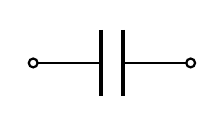
\begin{tikzpicture}
        \draw[thick] (3,0) to[C,o-o](5,0);
      \end{tikzpicture}
    \end{center}
  \item Act like a voltage source
  \item Unlike a battery, the voltage increases or decreases as the charge
    across the capacitor plates change.
  \end{itemize}
\end{frame}

\end{document}
